\section{Introduction}

\begin{wrapfigure}[18]{r}{0.4\textwidth}
   \vspace{-44pt}
   \centering
   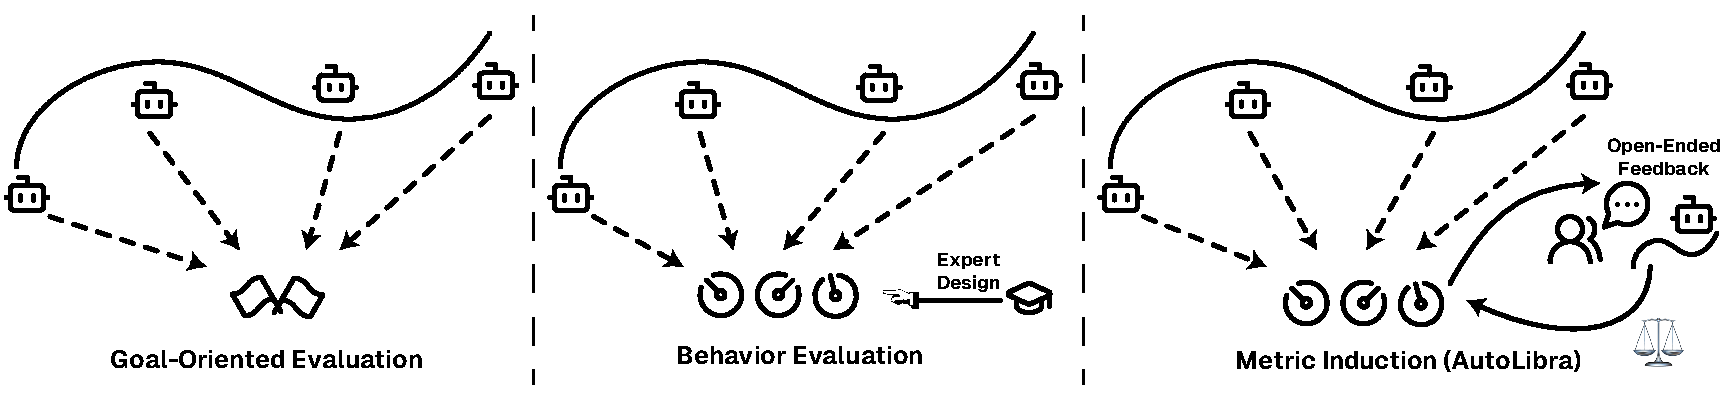
\includegraphics[width=0.4\textwidth]{figs/autolibra.pdf}
   \vspace{-10pt}
   \caption{AutoLibra provides behavioral evaluation on agent performance
    through automatic metric induction based on human feedback and agent trajectories.}
\end{wrapfigure}


Efficient human learners internalize open-ended feedback from others into self-regulation dimensions %metrics
\citep{pintrich2002development,nicol2006formative}.
These dimensions or ``metrics'' offer lenses for self-reflection on the
strengths and weaknesses of ourselves and ladders for self-improvement.
In this paper, we ask:
\textbf{can we automatically induce metrics to evaluate and improve agents from natural language feedback?} 

   
Current evaluation of large language model (LLM) agents and reward modeling often fall
into two paradigms: (1) goal-oriented evaluation --
\emph{whether the agents have fulfilled the given task},
\emph{e.g.} benchmarks \citep{zhouwebarena,jimenezswe,chan2024mle,paglieri2024balrog} and reward
modeling approaches \citep{pan2024autonomous,chen2025scaling,choudhury2025process}
and (2) behavior evaluation -- \emph{how well the agents do on heuristically designed dimensions},
\emph{e.g.} social agent and human-agent interaction benchmarks \citep{zhousotopia,shao2024collaborative}
and agent failure mode analysis \citep{pan2025why,zhang2023effects,yang2023behavioral}. 
Goal-oriented evaluation is often designed to be verifiable through considering, but it is not fine-grained
or comprehensive enough to diagnose agents' behavior problems or find the bottlenecks for improvements \citep{yehudai2025survey}.  
While behavior evaluation complements it, it requires manual design of the metrics either based on top-down heuristics
\citep{zhousotopia}, or thematic analysis of the agent's behavior \citep{shao2024collaborative,pan2025why}.
This manual design process is often time-consuming and labor-intensive through expert annotations and classifications. 

In this paper, we introduce AutoLibra \protect
\includegraphics[height=1em]{figs/scale.png},
a metric induction method as a new agent evaluation paradigm 
that mitigates the limitations of the current evaluation paradigms.
This method offers behavior evaluation for agents, with the following advantages:
(1) it provides multi-dimensional behavior evaluation that is fine-grained but requires no manual design of metrics,
(2) it could be applied to different kinds of agents and tasks, and 
(3) the metrics are fully explainable and interpretable by humans.

\begin{wrapfigure}[23]{l}{0.65\textwidth}
    \centering
    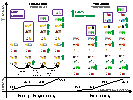
\includegraphics[width=0.65\textwidth]{figs/autolibra-teaser.pdf}
    \vspace{-10pt}
    \caption{AutoLibra iteratively discover new optimization targets throughout agent optimization process.}
    \label{fig:autolibra-training}
\end{wrapfigure}

Taking an inspiration from the code-theme steps of thematic analysis often conducted by human experts
in social sciences \citep{braun2006using},
we design the Extraction process of AutoLibra as a two step process:
(1) \emph{grounding}: ground every aspect of the human feedback into a slice of the whole agent trajectory,
and (2) \emph{clustering}: cluster the aspects of all trajectories into multiple clusters of similar behaviors
that can be summarized into metrics. For example, in the context of web agents, the grounding step will
``\textsf{If you find that the button is disabled, don't click it again}'' into a slice of the agent trajectory
``\texttt{action: click[1234]} \texttt{obs: no change} \texttt{action: click[1234]}''. Similar slices where 
agents repeated interact with disabled elements could be clustered into a metric \texttt{interact-valid-element}. 


The Evaluation process of AutoLibra is designed to provide a closed-loop feedback signal for both the Extraction process
and the LLM-as-a-Judge. The agent trajectories used in the Extraction process are scored by the LLM-as-a-Judge based
on the metrics induced by the Extraction process. The Evaluation process then tries to match the detected agent traits,
\emph{e.g.} \texttt{interact-valid-element}: \texttt{negative}, with the human feedback aspects.
In this way, we can meta-evaluate the \emph{coverage} of the detected traits, and the \emph{redundancy} of the metrics,
i.e. what proportion of the aspects in the human feedback are detected as agent traits,
and what proportion of the detected traits are not mentioned by humans. These two meta-metrics are used in selecting
metrics from candidates proposed in the Extraction process.



With AutoLibra, we aim to answer the following research questions:

\textbf{RQ1:} Can LLMs serve as a proxy for humans when being used in agent behavior thematic analysis,
    behavior evaluation, and meta-evaluating the LLM-as-a-Judge results?

\textbf{RQ2:}    What are the differences between the metrics induced by AutoLibra and the behavior evaluation
    metrics designed by human experts?

\textbf{RQ3:}  Is AutoLibra useful for improving the performance of agents by 
    providing fine-grained behavior evaluation for human agent engineers and agent learning algorithms?


With experiments on multiple agent domains, including collaborative agents \citep{shao2024collaborative}, social agents 
\citep{zhousotopia}, web agents \citep{zhouwebarena,he2024webvoyager}, and text game agents \citep{paglieri2024balrog,cloos2024babaaibreakrules}, 
we find that the performance of AutoLibra varies across different domains. 
However, it could induce fine-grained and interpretable metrics with high coverage and low redundancy on unseen human feedback.
We also find that new metrics can be iteratively discovered by AutoLibra through the agent optimization process,
and provide optimization signals that are useful for improving the performance of agents in different tasks.




